\chapter{Funcionalidades do MDArte}

Neste capítulo iremos explorar algumas funcionalidades que já existem no MDArte,
a fim de agilizar e simplificar o processo de desenvolvimento. Para tal
alteraremos os modelos de \texttt{CRUD} gerados automaticamente pelo
\texttt{MDArte}. Para evitar que as alterações feitas sejam sobrescritas por
engano, vá no diagrama de classe que descreve as entidades do Banco de Dados,
abra a especificação da classe \texttt{Estudante}, selecione a aba
\texttt{stereotypes} e remova o estereótipo \texttt{«Manageable»}.

\section{Campo com Autocomplete}

Nesta seção veremos como implementar um \texttt{autocomplete} para um
determinado campo de texto. Iremos transformar o campo \texttt{matricula} do
caso de uso \texttt{Consulta Estudante} em um campo com \texttt{autocomplete}.

O modelo inicial do caso de uso \texttt{Consulta Estudante} no  \texttt{CRUD}
para a entidade estudante pode ser visto na imagem \ref{modelo_consulta_estudante}:

\begin{figure}[H]
	\centering
	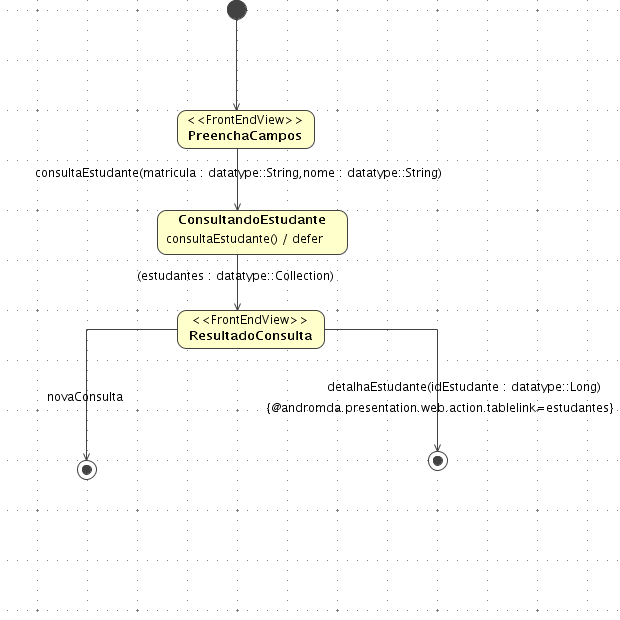
\includegraphics[width=350pt,height=300pt]{files/imgs/tutorial-mdarte-0028.png}
	\caption{Modelo do caso de uso Consulta Estudante.}
	\label{modelo_consulta_estudante}
\end{figure}

Abriremos a especificação da \texttt{transition} que sai da \texttt{front end
view} de nome \texttt{preencha os campos}, clicaremos no botão \texttt{edit}, no
\texttt{fieldset} \texttt{trigger}. Na aba \texttt{parameters}, da janela
\texttt{signal event specification}, que será aberta automaticamente, dê duplo
clique no nome do parâmetro \texttt{matricula} e será então aberta a
especificação do parâmetro. Selecione então a aba \texttt{tagged values},
selecione o \texttt{tagged value}
\texttt{@andromda.presentation.web.view.field.type} e clique no botão
\texttt{create value}. Selecione então a opção \texttt{autocomplete}, como na
imagem \ref{field_type_autocomplete}.

\begin{figure}[H]
	\centering
	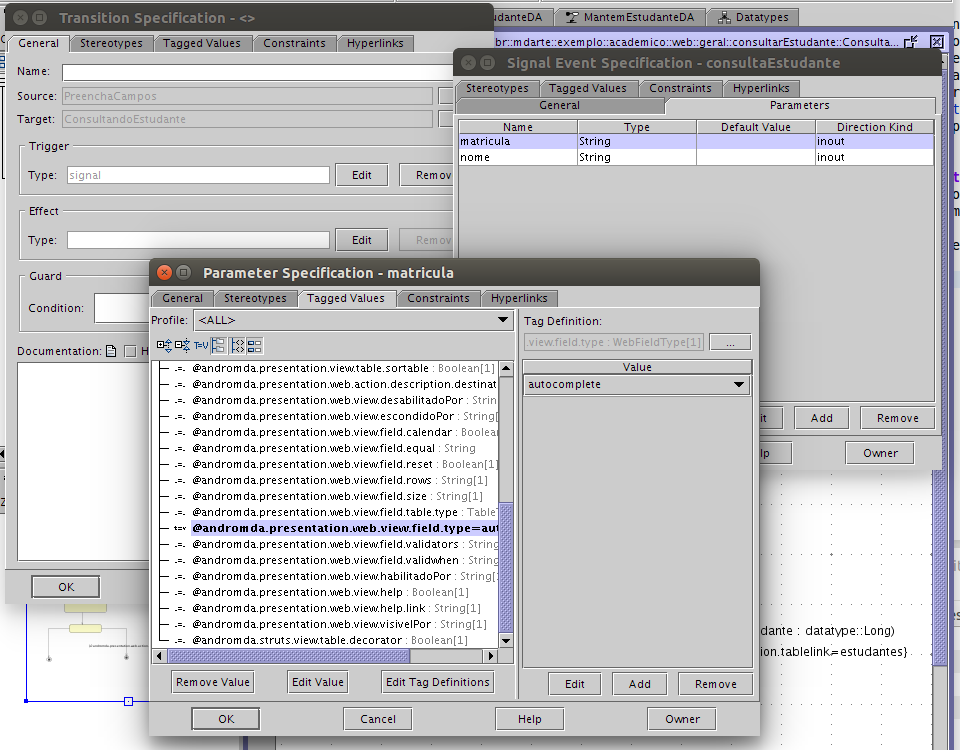
\includegraphics[width=350pt,height=300pt]{files/imgs/tutorial-mdarte-0027.png}
	\caption{Adicionando o field type 'autocomplete' à um campo da view.}
	\label{field_type_autocomplete}
\end{figure}

Agora executaremos o seguinte comando no terminal na raiz do projeto:
\begin{lstlisting}[language=bash]
maven mda -Dprojeto=sistemaacademico-geral-Estudante
\end{lstlisting}

Feito isto, o \texttt{MDArte} gerará automaticamente toda a estrutura
responsável por receber e tratar as requisições assíncronas para o preenchimento do
\texttt{autocomplete}, restando ao desenvolver apenas implementar no
\texttt{ControleImpl} a filtragem dos valores retornados, de acordo com o valor
do campo. Para isto, criaremos, na classe
\texttt{ConsultaEstudanteControleImpl}, um método seguindo o seguinte padrão 
\texttt{protected String[]
<nome-do-campo><nome-do-caso-de-uso>AutoComplete(java.lang.String query,
org.andromda.bpm4struts.ViewContainer container)}. Vejamos abaixo um exemplo de
implementação para o \texttt{autocomplete} do nosso campo de \texttt{matrícula}:

\lstinputlisting[language=java, frame=single, breaklines=true] {files/java/autocomplete.java}

Agora executaremos o seguinte comando para compilar e dar \texttt{deploy} no
\texttt{Sistema Acadêmico} :

\begin{lstlisting}[language=bash, frame=single, breaklines=true]
maven compile deploy
\end{lstlisting}

Feito isto, daremos \texttt{start} no \texttt{JBoss} e abriremos o sistema e
faremos login. Na tela \texttt{Preencha os Campos} do caso de uso
\texttt{Consulta Estudante} podemos agora verificar o \texttt{autocomplete}
funcionando, como na imagem \ref{exemplo_autocomplete}.

\begin{figure}[H]
	\centering
	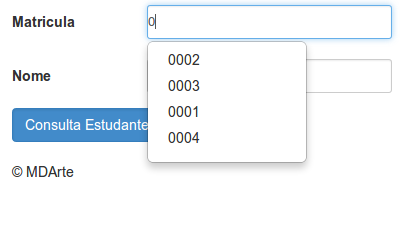
\includegraphics[width=350pt,height=300pt]{files/imgs/tutorial-mdarte-0029.png}
	\caption{Exemplo de autocomplete.}
	\label{exemplo_autocomplete}
\end{figure}
\section{Estratégia de paginação}

Estratégias de paginação foram criadas para comportar diferentes tipos de tabela
e paginação. Nas versões anteriores, a paginação era feita do mesmo jeito para
as tabelas Struts e Ajax porém elas tinham estruturas diferentes o que gerava
erros nas tabelas. Dessa forma, não poderíamos usar a tabela Ajax pois tinhamos
como prioridade ter a tabela Struts funcionando. Com as estratégias de paginação
podemos utilizar qualquer tipo de tabela sem ter que alterar a estrutura dos
DAOs e damos a opção para o desenvolvedor customizar a paginação do jeito que
quiser.

Nesta seção demonstraremos como utilizar estratégias de paginação. Primeiro,
apresentaremos a classe abstrata \texttt{PaginationStrategy}:

\lstinputlisting[language=java, frame=single, breaklines=true] {files/java/PaginationStrategy.java}

A classe abstrata \texttt{PaginationStrategy} é gerado no pacote util do
projeto. Nele você seta a página a ser obtida,  o número de linhas por
página e o número de páginas a serem retornadas pela \texttt{query} e
\texttt{criteria}.

Nela há a função \texttt{paginateResult} que possui duas assinaturas diferentes.
O desenvolvedor tem que implementar essas funções caso deseje criar a sua
própria estratégia. Um exemplo de implementação de estratégia é o
\texttt{PaginationSimple.java} que é utilizado para a paginação da tabela ajax.

\lstinputlisting[language=java, frame=single, breaklines=true] {files/java/PaginationSimple.java}

Além dessa estratégia, criamos outras duas: \texttt{PaginationDisplaytag} para as tabelas Struts e \texttt{NoPagination} caso não seja preciso de paginação.

A pasta em que sua implementação deve ser criada é
<projeto>/common/src/java/<pacote\_do\_projeto>/util e o import a ser feito é
\texttt{<pacote\_do\_projeto>.util.<nome>}.

Demonstramos um simples exemplo para instanciar uma estratégia abaixo:

\begin{lstlisting}[language=java, frame=single, breaklines=true]
	import br.mdarte.exemplo.academico.util.PaginationDisplaytag;
	import br.mdarte.exemplo.academico.util.Constantes;
	
	Integer pagina = ((Integer)request.getAttribute(Constantes.PARAMETRO_PAGINA)); //Struts 1
	Collection exemplos = ServiceLocator.instance().getExemploHandlerBI().recuperaExemplos(new PaginationDisplaytag(paginacao));
\end{lstlisting}
\section{Internacionalização}

Internacionalizar aplicações web é cada vez mais uma tarefa corriqueira de todo
desenvolvedor web e é um dos processos importantes para o aumento da
acessibilidade do sistema. O framework deve permitir mecanismo para facilitar a
utilização de diversas línguas. Para tal, foi construido um conjunto de
ferramentas para facilitar esse processo. A maioria dos frameworks web tem a sua
maneira particular de prover esse mecanismo, mas o que muita gente desconhece é
que existe uma forma padrão de fazer isso,  definida na especificação do Java EE, através da JSP Standard TagLibs.

O MDArte utiliza esse mecanismo e já provê ela configurada. Assim, a
especificação de novas linguas se torna uma tarefa ainda mais fácil.

Segue abaixo os passos para a definições de novas linguas.

\subsection{Mensagens}

Cada arquivo properties conterá todas as traduções do sistema. Todos os textos
do sistemas serão representados por uma \texttt{key}. Cada \texttt{key} e sua
respectiva mensagem, ou seja, \texttt{label} serão listadas em cada arquivo como
properties. Abaixo segue um exemplo:

\begin{lstlisting}[language=xml, frame=single, breaklines=true]
	label.key=Mensagem
\end{lstlisting}

Todas os recursos modelados no diagrama de atividades serão gerados com uma \texttt{key}.
Caso essa \texttt{key} não esteja no arquivo properties, o sistema utilizará a
\texttt{key} como \texttt{label} contudo sem o ponto.

Cada uma das possibilidades será abordada.

\subsubsection{Título de uma Página}

Todo título de página é gerado com uma key para o desenvolvedor possa definir no
custom-resources. 

\begin{lstlisting}[language=html, frame=single, breaklines=true]
	<tiles:put name="title" type="string">
    	<bean:message key="pagina.exemplo.title"/>
	</tiles:put>
\end{lstlisting}

\subsubsection{Campo ou Botão de uma Página}

Todo campo ou botão é gerado com uma key definida pelo o nome do caso de uso
somado com o nome do campo/botão. Segue abaixo um exemplo.

\begin{lstlisting}[language=html, frame=single, breaklines=true]
	<td class="field">
	<s:set name="__value" value="#session.form.nome"/>
	<div id="divnomeConsultaCursoUC" class="textfield field">
    	<label class="textfieldLabel" for="nome"><bean:message key="consulta.curso.uc.preencha.campos.consulta.curso.param.nome"/></label>
    	<s:textfield id="nomeConsultaCursoUC" name="nome" label="%{getText('consulta.curso.uc.preencha.campos.consulta.curso.param.nome')}" value="%{#session.form.nome}" title="" styleId="consultaCursoNome" />
</div>
\end{lstlisting}

\subsubsection{Exception}

Toda mensagem carregando uma \texttt{exception} também é substituída quando a
\texttt{key} na \texttt{exception} é encontrada no \texttt{custom-resource}.
Segue abaixo um exemplo.

\begin{lstlisting}[language=java, frame=single, breaklines=true]
	throw new Exception("ocorre.erro.esperado");

	throw new Exception("ocorre.erro.nao.esperado", exception);
\end{lstlisting}

Existem algumas funções que não interrompem a execução, mas possui o mesmo
efeito do \texttt{exception}. Segue abaixo um exemplo.

\begin{lstlisting}[language=java, frame=single, breaklines=true]
	saveErrorMessage(request, "informando.erro.key");
	saveWarningMessage(request, "informando.aviso.key");
	saveSuccessMessage(request, "informando.sucesso.key");
\end{lstlisting}

\subsubsection{Passagem de Parâmetros}

Existe a possibilidade de passar parâmetros para a mensagem. Será passando um
\texttt{array} de \texttt{string} e na mensagem existirá marcadores informando
onde será colocado o conteúdo do \texttt{array}.

\textbf{Exemplo:}

\texttt{custom-resources.properties}

\begin{lstlisting}[language=xml, frame=single, breaklines=true]
	label.key=Mensagem com parametro {0}
\end{lstlisting}

\texttt{Código:}

\begin{lstlisting}[language=java, frame=single, breaklines=true]
	String[] parametro = new String[1];
	parametro[0] = "param1";
	saveErrorMessage(request, "label.key", parametro);
\end{lstlisting}

Assim será exibido a seguinte mensagem: \texttt{Mensagem com
parametro param1}

\subsection{Arquivo de Configurações}

Edite o arquivo \textbf{<DiretorioProjeto>}/mda/conf/andromda.xml e na
propriedade \texttt{languages} informe os locales que serão utilizados.

Exemplo:

\begin{lstlisting}[language=xml, frame=single, breaklines=true]
	<property name="languages">pt,en,fr</property>
\end{lstlisting}

Após a geração utilizando essa configuração será criado novos três arquivos: 

\begin{lstlisting}[language=xml, frame=single, breaklines=true]
	custom-resources_en.properties
	custom-resources_pt.properties
	custom-resources_fr.properties
\end{lstlisting}

Além do arquivo já criado no geração da aplicação:

\begin{lstlisting}[language=xml, frame=single, breaklines=true]
	custom-resources.properties
\end{lstlisting}

Automaticamente o sistema irá detectar qual locale do browser que o usuário está
utilizando e utilizará o locale correto. Caso não exista o locale pré-definido,
o sistema utilizará o \texttt{custom-resources} padrão.

O desenvolvedor poderá forçar um locale específico pelo código. Exemplo: 

\begin{lstlisting}[language=java, frame=single, breaklines=true]
	//Recuperando o Locale
	Locale locale = (Locale) request.getSession().getAttribute("org.apache.struts.action.LOCALE");

	//Definindo um Locale
	request.getSession().setAttribute("org.apache.struts.action.LOCALE", new Locale("pt", "BR"));
\end{lstlisting}

\section{Pontos de decisão}

Pontos de decisão são criados quando sua aplicação precisa tomar decisões
dependendo do resultado de uma ação prévia. Utilizamos uma forma de modelagem
ofericida pela especificação UML.

Nela você desenha uma linha de transição a partir da ação conectando-a ao ponto
de decisão. Um ponto de decisão é desenhado como um losango em UML. Já que uma
decisão tem pelo menos dois resultados diferentes, o ponto de decisão terá
múltiplas transições para diferentes ações.

Usaremos como exemplo para introduzir um ponto de decisão o seguinte diagrama de
atividades:

\begin{figure}[H]
	\centering
	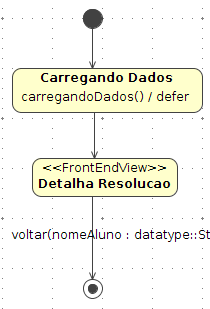
\includegraphics[scale=0.75]{files/imgs/decision-point-00.png}
	\caption{Modelo inicial do exemplo}
	\label{modelo_inicial_ponto_decisao}
\end{figure}

Criamos um ponto de decisão e colocamos uma transição do estado
\textbf{Carregando Dados} para o ponto de decisão:

\begin{figure}[H]
	\centering
	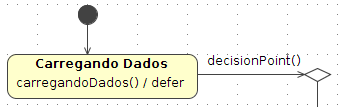
\includegraphics[scale=0.75]{files/imgs/decision-point-01.png}
	\caption{Criando o ponto de decisão}
	\label{criando_ponto_decisao}
\end{figure}

Em seguida na classe de controle do diagrama de atividades criamos uma função
chamada \texttt{decisionPoint}:

\begin{figure}[H]
	\centering
	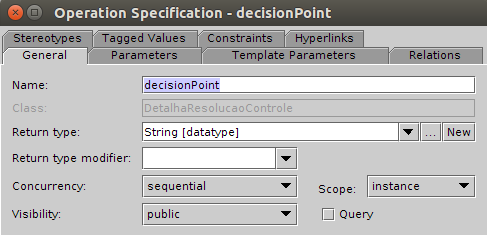
\includegraphics[scale=0.75]{files/imgs/decision-point-02.png}
	\caption{Criando função do ponto de decisão}
	\label{funcao_ponto_decisao}
\end{figure}

Na transição para o ponto de decisão, alteramos a \texttt{trigger} e colocamos o
tipo dela como \texttt{call} e a operação como \texttt{decisionPoint}:

\begin{figure}[H]
	\centering
	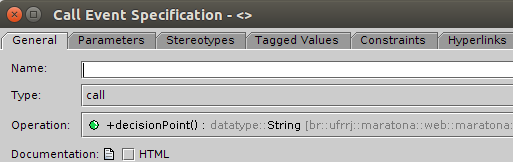
\includegraphics[scale=0.75]{files/imgs/decision-point-03.png}
	\caption{Colocando a função na transição}
	\label{funcao_transicao}
\end{figure}

O próximo passo é passar o início da transição que ia de \textbf{Carregando
Dados} para \textbf{Detalha Resolucao} para o ponto de decisão e criar uma
transição do ponto de decisão para o estado final.

\begin{figure}[H]
	\centering
	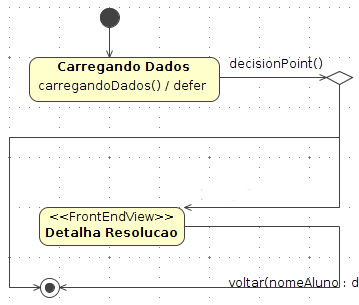
\includegraphics[scale=0.75]{files/imgs/decision-point-04.png}
	\caption{Colocando a função na transição}
	\label{ponto_decisao_com_transicoes}
\end{figure}

Em seguida devemos criar a condição de guarda dessas transições. Na aba
\texttt{General}, clicamos no botão \texttt{Edit} da seção \texttt{Guard}:

\begin{figure}[H]
	\centering
	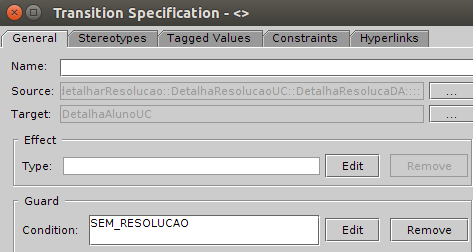
\includegraphics[scale=0.75]{files/imgs/decision-point-05.png}
	\caption{Abrindo a transição}
	\label{abrindo_transição}
\end{figure}

Agora especificamos o nome da condição de guarda e a condição em si. Ambos tem
que ter o mesmo nome:

\begin{figure}[H]
	\centering
	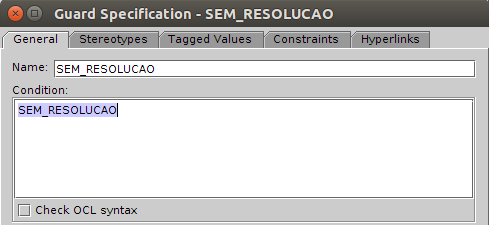
\includegraphics[scale=0.75]{files/imgs/decision-point-06.png}
	\caption{Especificando a condição de guarda}
	\label{condicao_de_guarda}
\end{figure}

Fazemos o mesmo para a outra transição e o modelo final é o seguinte:

\begin{figure}[H]
	\centering
	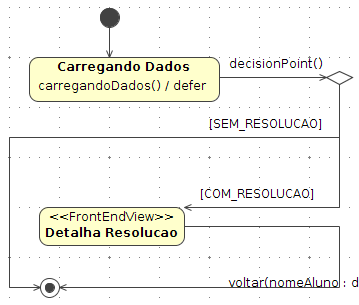
\includegraphics[scale=0.75]{files/imgs/decision-point-07.png}
	\caption{Modelo final}
	\label{modelo_final}
\end{figure}

Agora temos que implementar a função \texttt{decisionPoint}. Ela tem que
retornar uma String que seja uma das condições de guarda especificadas no
modelo. Exemplo de código:

\begin{lstlisting}[language=java, frame=single, breaklines=true]
	public String decisionPoint(DecisionPointForm form, ViewContainer container) throws Exception
	{
		if (form.getIdResolucao() != null) {
			return "COM_RESOLUCAO";
		}
		else {
			return "SEM_RESOLUCAO";
		}
	}
\end{lstlisting}
\section{Tabela assíncrona (JTable)}

Nesta seção veremos como implementar uma tabela \texttt{assíncrona}
(\texttt{JTable}) usando o \texttt{MDArte}. Para tal, vamos considerar como
ponto de partida o modelo do caso de uso \texttt{Consulta Estudante} conforme as
alterações feitas no tópico anterior. Certifique-se de ter removido o
estereótipo \texttt{«Manageable»} da classe \texttt{Estudante} no diagrama de
classes que descreve a \texttt{Camada de domínio}, a fim de evitar que o
\texttt{CRUD} seja re-gerado, sobrescrevendo assim as alterações que faremos.

Veremos agora, por subseções, algumas das funcionalidades disponíveis na tabela
assíncrona.

\subsection{Implementando filtragem assíncrona da tabela}
Nesta seção veremos como criar uma action ajax que reflita nos dados exibidos
por uma tabela ajax. A título de exemplo, faremos uma tela com um formulário e
um botão que, uma vez clicado, recarregará a tabela filtrando-a de acordo com os
dados do formulário. Tomaremos como base a tabela criada no exemplo de criação
de tabelas.

O modelo portanto começará assim:

\begin{figure}[H]
	\centering
	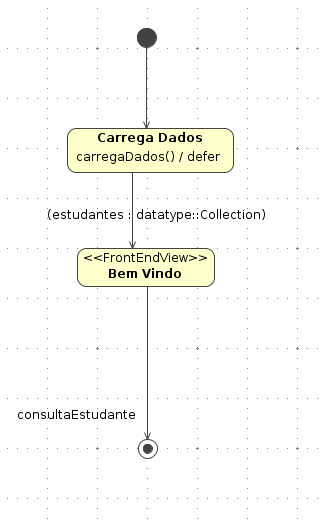
\includegraphics[width=180pt,height=260pt]{files/imgs/tutorial-mdarte-0040.png}
	\caption{Modelagem da filtragem assíncrona da tabela.}
	\label{modelando_filtragem_assincrona}
\end{figure}

Modelaremos então uma \texttt{transition} saindo da \texttt{FrontEndView} que
contém a nossa tabela e retornando para a mesma \texttt{view}, que será
interpretada pelo \texttt{MDArte} como uma ação assíncrona na \texttt{view}.
Abriremos então sua especificação e iremos na aba \texttt{tagged values} e
selecionaremos o \texttt{tagged value}
\texttt{@andromda.presentation.web.action.async.table} e daremos a ele o valor
\texttt{[nome-da-tabela]} (\texttt{estudantes}, nesse caso), esse \texttt{tagged
value} indica qual tabela será afetada pela ação assíncrona, nos permitindo ter
mais de uma de tabela assíncrona na mesma tela, tendo \texttt{actions} que
afetem somente uma tabela sem afetar a outra. Iremos então na aba
\texttt{general} e clicaremos no botão \texttt{edit} no \texttt{fieldset}
\texttt{'trigger'}, daremos o nome que desejarmos o \texttt{trigger} criado, no
exemplo fo idado o nome de \texttt{“filtrar”}, e selecionaremos seu tipo como
\texttt{signal}. Iremos então na aba \texttt{parameters}, ainda na especificação
do \texttt{trigger} e criaremos os parâmetros necessários para o processamento
da requisição, neste exemplo colocaremos só os parâmetros \texttt{matrícula} e
\texttt{nome}, a título de ilustração, e definiremos seus tipos como
\texttt{String}.

O modelo ficará assim:
\begin{figure}[H]
	\centering
	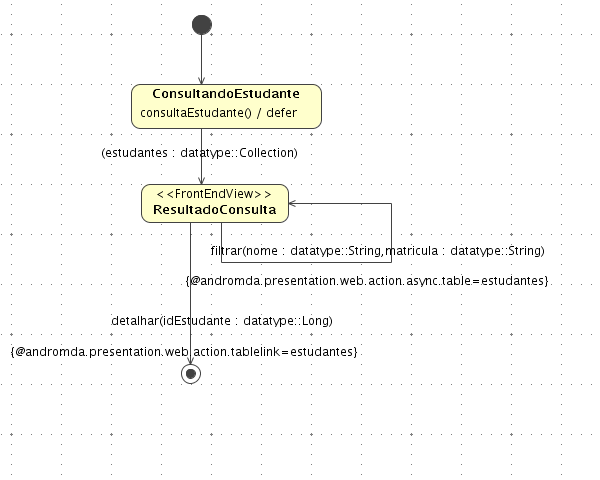
\includegraphics[width=340pt,height=300pt]{files/imgs/tutorial-mdarte-0036.png}
	\caption{Modelagem da filtragem assíncrona da tabela.}
	\label{modelando_filtragem_assincrona}
\end{figure}

Executaremos agora o seguinte comando para validar o modelo e regerar o
sistema:
\begin{lstlisting}[language=bash, frame=single, breaklines=true]
maven mda -Dprojeto=sistemaacademico-geral-Estudante
\end{lstlisting}

Agora adaptaremos, no \texttt{ControleImpl}, os métodos responsáveis pelo
carregamento da tabela, com a assinatura \texttt{public final Collection
load[nome-da-view][nome-da-tabela]Table}, e pelo retorno do número máximo de
elementos na mesma, com a assinatura \texttt{public final Integer
get[nome-da-view][nome-da-tabela]TableLength}, a fim de implementarmos o filtro.
Cada parâmetro da \texttt{trigger} pertencente à \texttt{transition} modelada
será adicionado, em ordem, à lista de parâmetros de cada método, logo antes do
parâmetro \texttt{ViewContainer container}. De acordo com o nosso exemplo, o
código ficará assim:
\lstinputlisting[language=java, frame=single, breaklines=true]{files/java/JTableFiltro.java}

Executaremos agora o seguinte comando para compilar e dar \texttt{deploy} no
sistema:
\begin{lstlisting}[language=bash, frame=single, breaklines=true]
maven compile deploy
\end{lstlisting}

Restartando o servidor e abrindo o caso de uso \texttt{Consulta Estudante},
veremos o resultado do que fizemos:
\begin{figure}[H]
	\centering
	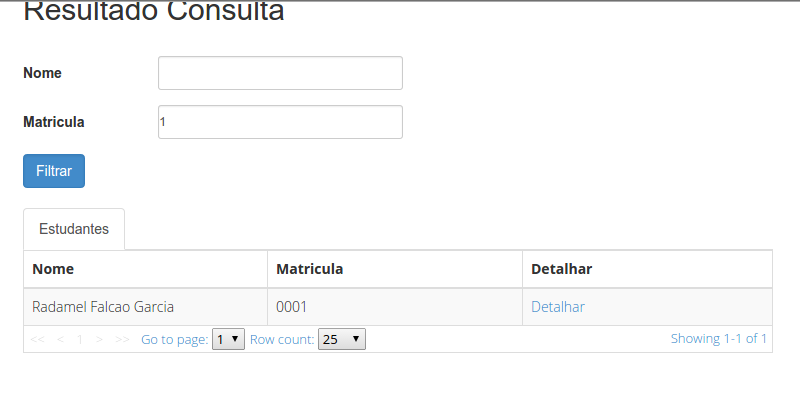
\includegraphics[width=340pt,height=300pt]{files/imgs/tutorial-mdarte-0042.png}
	\caption{Modelagem da filtragem assíncrona da tabela.}
	\label{modelando_filtragem_assincrona}
\end{figure}

\section{Criação de Componente customizado}

Nesta seção veremos como criar um campo customizado em uma tela. Iremos partir
do modelo de \texttt{CRUD} gerado automaticamente pelo \texttt{MDArte}, para a
entidade \texttt{Estudante}, e faremos as alterações necessárias para a criação
de um novo componente. O componente a ser desenvolvido, somente a título de
exemplo, será um campo texto com máscara para \texttt{CPF}.

Podemos ver o estado inicial do modelo na imagem \ref{modelo_consulta_estudante_custom}.

\begin{figure}[H]
	\centering
	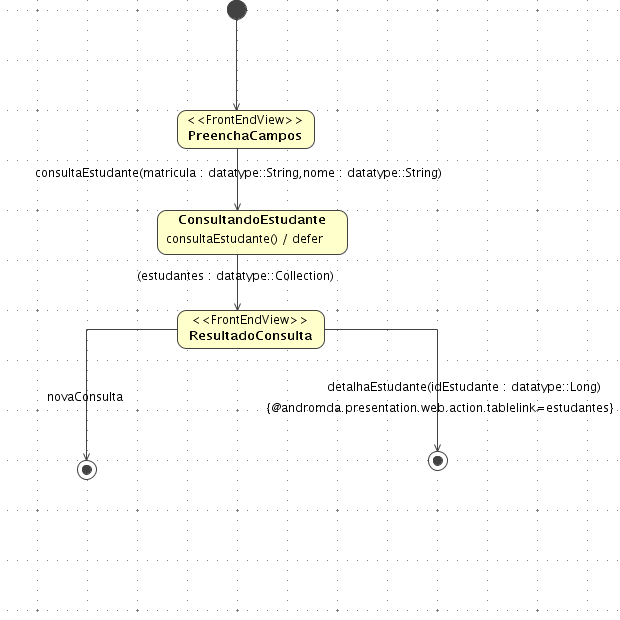
\includegraphics[width=350pt,height=300pt]{files/imgs/tutorial-mdarte-0028.png}
	\caption{Modelo do caso de uso Consulta Estudante.}
	\label{modelo_consulta_estudante_custom}
\end{figure}

Abriremos então a especificação da \texttt{transition}
\texttt{'consultaEstudante'}, clicaremos no botão \texttt{'edit'}, no
\texttt{fieldset} \texttt{'trigger'}, selecionaremos então a aba
\texttt{'parameters'}, da janela aberta quando clicamos o botão anterior, e
clicaremos então no botão \texttt{add}.

Preencheremos então os dados do campo conforme a imagem
\ref{dados_campo_custom_cpf}, SEM, no entanto, clicar no botão \texttt{Ok}.

\begin{figure}[H]
	\centering
	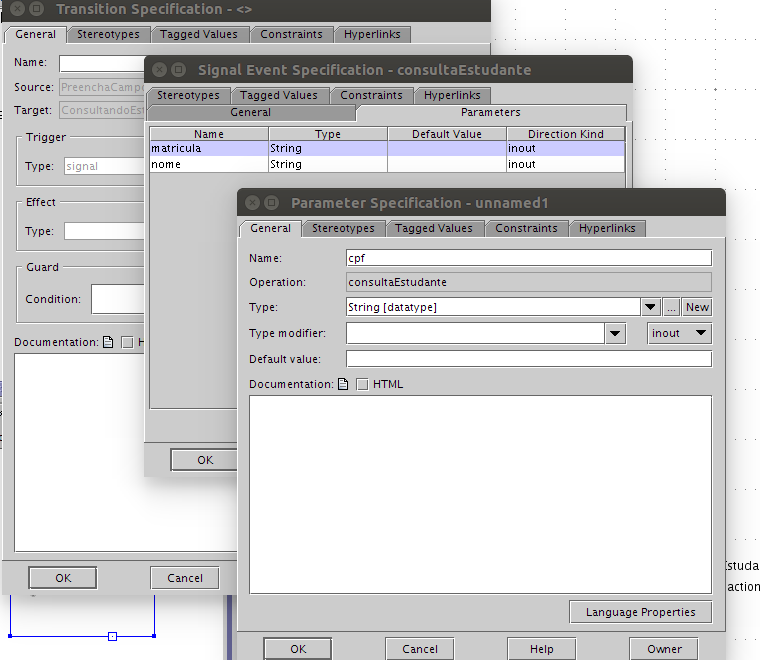
\includegraphics[width=350pt,height=300pt]{files/imgs/tutorial-mdarte-0033.png}
	\caption{Dados do campo 'cpf'.}
	\label{dados_campo_custom_cpf}
\end{figure}

Ainda na mesma janela, selecionaremos a aba \texttt{tagged values},
selecionaremos o \texttt{tagged value} 
\texttt{@andromda.presentation.web.view.field.type}, clicaremos no botão
\texttt{create value} e selecionaremos a opção \texttt{'custom'}, no campo
\texttt{combobox} que será exibido, como na imagem \ref{parametro_cpf_custom}.

\begin{figure}[H]
	\centering
	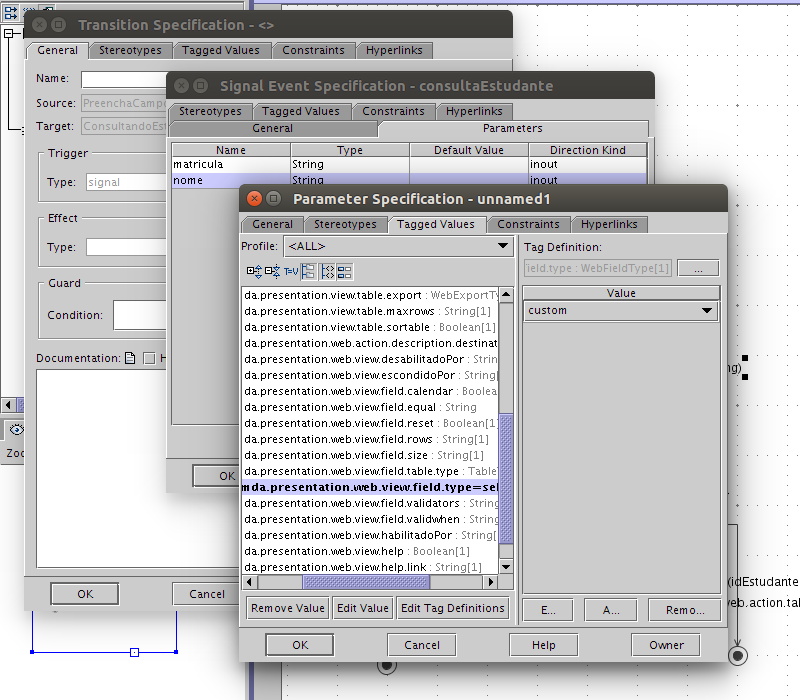
\includegraphics[width=350pt,height=300pt]{files/imgs/tutorial-mdarte-0034.png}
	\caption{Selecionando tipo custom para o campo 'cpf'.}
	\label{parametro_cpf_custom}
\end{figure}

Salvaremos então o modelo e digitaremos os seguintes comandos para regerar o
modelo:

\begin{lstlisting}[language=bash, frame=single, breaklines=true]
maven mda -Dprojeto=sistemaaacademico-geral-Estudante
\end{lstlisting}

Feito isto, o \texttt{MDArte} gerará um arquivo no padrão
\texttt{<nome-do-campo>.jsp}, neste caso, \texttt{cpf.jsp}, no caminho
\texttt{<nome-sistema>/web/<modulo-web>/src/jsp/<caminho-do-pacote-base>/web/<modulo-web>/<nome-caso-de-uso>},
mas você também pode encontrá-lo, no eclipse, através do comando
\texttt{ctrl+shift+r}, digitando o nome do arquivo na janela que é aberta por
esse comando.

Aberto o arquivo, adicionaremos a este o seguinte código \texttt{jsp}:

\lstinputlisting[language=html, frame=single, breaklines=true]{files/jsp/cpf.jsp}

O \texttt{html} adicionado será importado para a tela do sistema no espaço do
formulário dedicado ao campo \texttt{cpf}.

Adicionado o \texttt{jsp} do nosso componente, uma vez que se trata de um campo
de texto com um determinado comportamento (formatar a entrada no modelo do CPF),
precisamos agora adicionar um mecanismo de controle para o comportamento do
campo. Para tal, utilizaremos o \texttt{framework} para \texttt{javascript}
JQuery, uma vez que este já vem com o \texttt{MDArte}, além do fato de o
\texttt{JQuery} já possuir uma funcionalidade nativa que faça isso.

Para adicionar código \texttt{Javascript} manualmente a uma \texttt{view}
precisamos abrir o arquivo \texttt{<nome-da-view>-impl.js}, no mesmo caminho
do arquivo \texttt{jsp} alterado acima. O arquivo alterado é destinado ao código
adicionado pelo desenvolvedor para customizar o comportamento da aplicação, não
sendo sobrescrito durante a geração. Certifique-se, portanto, de estar
adicionando o seu código nestes pontos de implementação, a fim de não perdê-lo
na próxima geração.

Adicionaremos agora o seguinte código \texttt{JavaScript} ao arquivo
\texttt{preencha-campos-impl.js}:

\lstinputlisting[language=c, frame=single, breaklines=true]{files/js/preencha-campos-impl.js}